\noindent The kinematics of a ship is expressed in the middle of the ship in a ship fixed coordinate system, rotated around the Earth-fixed coordinate system $x_0$, $y_0$ by the heading angle $\Psi$ as shown in \autoref{fig:reference_frames}. 
\begin{figure}[h!]
    \centering
    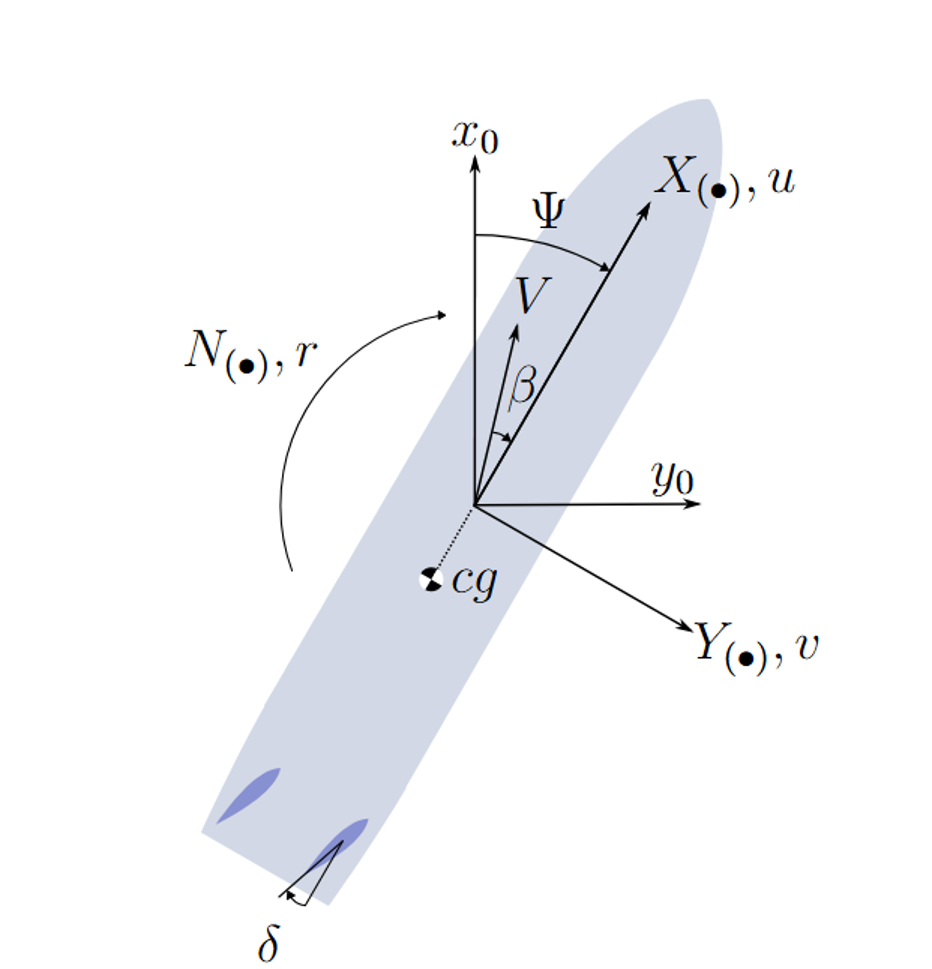
\includegraphics[width=6cm, height=6cm]{figures/reference_frames.png}
    \caption{Ship velocities and forces in the Earth-fixed and ship-fixed coordinate systems.}
    \label{fig:reference_frames}
\end{figure}
Forces and motions are expressed in three degrees of freedom, that is, surge $X$, sway $Y$, and yaw $N$. During a ship's maneuvering, since the forces do not depend on the position ($x_0,y_0$) or heading $\Psi$, the kinematics and motion equations of the ship can be expressed as a function of the velocity vector $\pmb{\bm{\upsilon}}$ as
% \begin{equation}
%     \label{eq:upsilon}
%     %\upsilon = \left[\begin{matrix}u\\v\\r\end{matrix}\right]
%     \pmb{\bm{\upsilon}} = \left[\begin{matrix}u\\v\\r\end{matrix}\right]
% \end{equation}
% The equation of motion can thus be expressed as \autoref{eq:eom}
\begin{equation}
    \label{eq:eom}
    \mathbf{F} = \mathbf{M}  \pmb{\bm{\dot{\upsilon}}}, \hspace{1cm}
    \pmb{\bm{\upsilon}} = \left[\begin{matrix}u\\v\\r\end{matrix}\right]
\end{equation}
where $\pmb{\bm{\dot{\upsilon}}}$ is the acceleration vector, $\mathbf{M}$ is the system inertia matrix and $\mathbf{F}$ is the total force vector.
% The velocity transition can thus be expressed as
% \begin{equation}
%     \label{eq:acc}
%     \pmb{\bm{\dot{\upsilon}}} = \mathbf{M}^{-1}\mathbf{F}
% \end{equation}
The total forces can be divided into the Coriolis–centripetal matrix $\mathbf{C}$ and the damping force vector $\mathbf{D}$ \citep{fossenHandbookMarineCraft2011}, while the control forces from the rudder and propeller are included in the $\mathbf{D}$ matrix as follows,
\begin{equation}
    \label{eq:C_expanded}
    \mathbf{C} = \left[\begin{matrix}0 & - m r & Y_{\dot{r}} r + Y_{\dot{v}} v - m r x_{G}\\m r & 0 & - X_{\dot{u}} u\\- Y_{\dot{r}} r - Y_{\dot{v}} v + m r x_{G} & X_{\dot{u}} u & 0\end{matrix}\right], \hspace{0.3cm}
    \mathbf{D} = \left[\begin{matrix}X_{D}\\Y_{D}\\N_{D}\end{matrix}\right]
\end{equation}
% \begin{equation}
%     \label{eq:D}
%     \mathbf{D} = \left[\begin{matrix}X_{D}\\Y_{D}\\N_{D}\end{matrix}\right]
% \end{equation}
where the added masses  $X_{\dot{u}},Y_{\dot{v}},Y_{\dot{r}},N_{\dot{v}},N_{\dot{r}} < 0$, then the total force vector $\mathbf{F}$ can now be expressed as:
\begin{equation}
    \label{eq:F_expanded}
    %F = \mathbf{D} + \mathbf{\tau_{wave}} + \mathbf{\tau_{wind}} + \mathbf{\tau} + \left[\begin{matrix}m r v - r \left(Y_{\dot{r}} r + Y_{\dot{v}} v - m r x_{G}\right)\\X_{\dot{u}} r u - m r u\\- X_{\dot{u}} u v - u \left(- Y_{\dot{r}} r - Y_{\dot{v}} v + m r x_{G}\right)\end{matrix}\right]
\mathbf{F} = - \mathbf{C} \upsilon + \mathbf{D} =
\left[\begin{matrix}
X \\
Y \\
N \\
\end{matrix}\right]
=
\left[\begin{matrix}X_{D} - Y_{\dot{r}} r^{2} + m r^{2} x_{G} + r v \left(- Y_{\dot{v}} + m\right)\\Y_{D} + r u \left(X_{\dot{u}} - m\right)\\N_{D} + r u \left(Y_{\dot{r}} - m x_{G}\right) + \underbrace{u v \left(- X_{\dot{u}} + Y_{\dot{v}}\right)}_{\text{Munk moment}} \end{matrix}\right]
\end{equation}
where $u v \left(- X_{\dot{u}} + Y_{\dot{v}}\right)$ in the yawing moment $N$ is the so called Munk moment \citep{fossenHandbookMarineCraft2011}; $r u \left(X_{\dot{u}} - m\right)$ in the sway force $Y$ has the apparent centrifugal force from added mass and rigid body mass with $X_{\dot{u}}<0$, so that both added mass and rigid body mass create the centrifugal force acting outward in the turn. Both the added mass and rigid body mass will thus act to starboard on a port turn.
% \begin{equation}
%     \label{eq:upsilon1d}
% \mathbf{F} = - \mathbf{C} \upsilon + \mathbf{D}
% \end{equation}

For the calculation of acceleration $\pmb{\bm{\dot{\upsilon}}}$ in \autoref{fig:reference_frames}, the mass matrix $\mathbf{M}$ and its inverse can be calculated according to \citet{fossenHandbookMarineCraft2011} as shown in, 
\begin{equation}
    \label{eq:M_expanded}
    \mathbf{M} = \left[\begin{matrix}- X_{\dot{u}} + m & 0 & 0\\0 & - Y_{\dot{v}} + m & - Y_{\dot{r}} + m x_{G}\\0 & - N_{\dot{v}} + m x_{G} & I_{z} - N_{\dot{r}}\end{matrix}\right],
   % \frac{1}{\mathbf{M}} = \left[\begin{matrix}\frac{1}{- X_{\dot{u}} + m} & 0 & 0\\0 & \frac{- I_{z} + N_{\dot{r}}}{S} & \frac{- Y_{\dot{r}} + m x_{G}}{S}\\0 & \frac{- N_{\dot{v}} + m x_{G}}{S} & \frac{Y_{\dot{v}} - m}{S}\end{matrix}\right]
\end{equation}
% \begin{equation}
%     \label{eq:M_inv}
%     \frac{1}{\mathbf{M}} = \left[\begin{matrix}\frac{1}{- X_{\dot{u}} + m} & 0 & 0\\0 & \frac{- I_{z} + N_{\dot{r}}}{S} & \frac{- Y_{\dot{r}} + m x_{G}}{S}\\0 & \frac{- N_{\dot{v}} + m x_{G}}{S} & \frac{Y_{\dot{v}} - m}{S}\end{matrix}\right]
% \end{equation}
% the helper variable $S = I_{z} Y_{\dot{v}} - I_{z} m - N_{\dot{r}} Y_{\dot{v}} + N_{\dot{r}} m + N_{\dot{v}} Y_{\dot{r}} - N_{\dot{v}} m x_{G} - Y_{\dot{r}} m x_{G} + m^{2} x_{G}^{2}$.
% \begin{equation}
%     \label{eq:S}
%     S = I_{z} Y_{\dot{v}} - I_{z} m - N_{\dot{r}} Y_{\dot{v}} + N_{\dot{r}} m + N_{\dot{v}} Y_{\dot{r}} - N_{\dot{v}} m x_{G} - Y_{\dot{r}} m x_{G} + m^{2} x_{G}^{2}
% \end{equation}
%\vspace{0.5cm}

